\documentclass[11pt,a4paper]{scrartcl}
%{{{ general stuff
\usepackage[a4paper,bindingoffset=0.2in,%
            left=1in,right=1in,top=1in,bottom=1in,%
            footskip=.25in]{geometry}
\usepackage[english]{babel}
\usepackage[utf8]{inputenc}
\usepackage[T1]{fontenc}
\usepackage{cite}
\usepackage[hidelinks]{hyperref}
\usepackage{float} % use H in figure placement
% \pagenumbering{gobble}

%}}}
%{{{ graphics
\usepackage{graphicx} % Bilder
\usepackage{tikz, pgfplots}
\pgfplotsset{compat=1.14}
%}}}
%{{{ math
\usepackage{mathrsfs} % mathcal and mathscr
\usepackage{mathtools, amssymb, amsthm}
\usepackage{bm} % cool bold symbols
%}}}
% a todo command===============================================================
\usepackage[ruled]{algorithm2e}
\newcounter{todocounter}
\newcommand{\todo}[2][noisnotdefined]{
 \marginpar{\fcolorbox{black}{orange}{\footnotesize\textbf{todo}}
 \ifthenelse{\equal{#1}{noisnotdefined}}{}{\textcolor{black}{\newline\tiny #1}}}
 \textbf{\ifthenelse{\equal{#2}{.}}
   {\fcolorbox{orange}{white}{\textcolor{orange}{$\maltese$}}}{{\textcolor{orange}{#2}}}}
 \refstepcounter{todocounter}}

%===============================================================================

\date{\today}
\title{Really Good Title}
\subtitle{Genetic Algorithms and Evolutionary Computing Project}
\author{Felix Bartel and D\'avid Kerekes}


\begin{document}

\maketitle
\todo{think about good title}

\section{Introduction}

In this project we explore some properties of neuroevolution, the technique of applying a genetic algorithm to a neural network \cite{Garis90geneticprogramming} \cite{Sims94evolving3d}.

Undoubtedly, the neural network architecture has been the star of the machine learning resurgence of the past few years. It's provable property of being an universal function approximator makes it a sensible choice for various applications. The main algorithm used for training, backpropagation however is subject to an array of criticism from authors (and even from Hinton himself), and there are various attempts at improving or replacing it \cite{zhang2007hybrid, riedmiller1993direct, montana1989training}.

A big advantage of the neuroevolution scheme is that for a series of different inputs a single scalar indicator of performance is sufficient to optimize a neural network for a certain task.
This can for instance be given by the outcome of a game.
Our game of choice is Blobby Volley 2 which is an open source, simple two-dimensional volleyball game written in C++ with lua support. Example picture in figure \ref{fig:screenshot}.

\begin{figure}[H]
\center
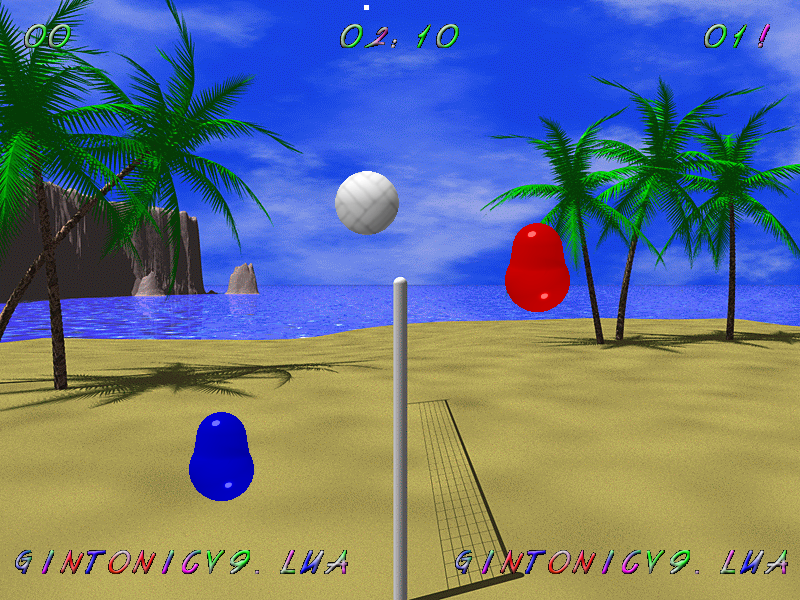
\includegraphics[width=0.4\textwidth]{img/screenshot.png}
\caption{Screenshot of the game.}
\label{fig:screenshot}
\end{figure}

\section{Training environment}

A scene from the game could be described by the $x$- and $y$-coordinates of the players and the ball, their corresponding velocities and the current number of ball contacts.
These arguments or a subset of them can then be used as input for the neural network.
The output should correspond to the possible movement options of the player, which consists of going right, going left, or jumping.
Assuming the layers of the neural network have $n_1,\dots,n_L$ nodes we then have to optimize \(N = \sum_{l=1}^{L-1} (n_l+1) \, n_{l+1}\) number of variables.

The game comes bundled with a number of bots with different styles, that are designed to pose a challenge to a wide range of human opponents. In order to define a clean ranking between them, we recorded the score of all possible lineups (figure \ref{tab:bot_vs_bot}).
\todo{explain the table}

\begin{figure}[H]
\begin{tabular}{c|ccccccc}
vs. &
\texttt{Axji-0-2} &
\texttt{COM\_11} &
\texttt{GintonicV9} &
\texttt{Hypo14} &
\texttt{reduced} &
\texttt{Union} &
\texttt{trainer} \\
\hline
\texttt{Axji-0-2} & - & 0 & 0 & 4 & 0 & 0 & 10 \\
\texttt{COM\_11} & 21 & - & 9 & 19 & 6 & 16 & 20 \\
\texttt{GintonicV9} & 21 & 12 & - & 19 & 6 & 16 & 20 \\
\texttt{Hypo14} & 17 & 2 & 2 & - & 2 & 5 & 15 \\
\texttt{reduced} & 21 & 19 & 15 & 19 & - & 19 & 21 \\
\texttt{Union} & 21 & 14 & 5 & 16 & 2 & - & 20 \\
\texttt{trainer} & 11 & 0 & 1 & 6 & 0 & 1 & -
\end{tabular}
\label{tab:bot_vs_bot}
\caption{Scores of bots competing against each other}
\end{figure}

We implemented our own bot marked \texttt{trainer} to act as an initial trainer for the network.
This trainer is easier to defeat than the other built-in players.
The simplification gives the evolutionary algorithm the opportunity to start optimizing the neural network in a valid direction, without introducing additional factors to the fitness score.

\section{Implementation}
The genotype-representation of the network is accomplished through python objects. This allows a straightforward implementation of a wide variety of genetic operators. Since our algorithm is constrained overwhelmingly by evaluation time, these inefficient but easy to modify structures do not impact performance.
As the evaluation of the population is time-consuming, we do this in a thread-parallel fashion, allowing us to exploit multiple high core-count machines at our disposal. In order to achieve this, we modified the original game by replacing the graphics and sound modules with dummies.

\section{Initial genetic algorithm}
Here we describe our starting point for the genetic algorithm. All subsequent versions are based off of this variant, with not mentioned details staying the same.

\subsection{Network architecture}

For the whole experiment, we fixed the size of the neural network to $6$ input nodes, one hidden layer with $7$ nodes and $2$ output nodes. As can be seen later, this proved sufficient for a surprisingly high performance by the network. The input nodes got fed with the x and y positions of the player, it's relative position compared to the ball, and the velocity vector of the ball.
The output nodes consisted of two neurons with tanh activations, one responsible for going left or right in the next timestep (if the output was below or above of threshold values $t_l = 0.49, t_r = 0.51$) and the other for jumping (above threshold $t_j = 0.7$).

\subsection{Scheme}
The algorithm worked with a population size of 100, with 150 offspring after crossover. Our survivor selection strategy was elitism, selecting from the pool of children plus the 10 best parents from the last generation.

The fitness function was the normalized point difference after $21$ serves.

\subsection{Mutation}
Mutation is accomplished by adding Gaussian noise to a subset of all weights and biases. We selected an individual for mutation with a probability of $0.7$, which then had a per-neuron mutation rate of $0.5$, and a sigma of $0.01$.

\subsection{Crossover}
As crossover we randomly mixed the nodes with belonging weights and biases of two networks and chose the parents via the fitness proportional roulette wheel selection.


\subsection{Numerical tests}
We trained six networks, each against a different bot. We test the generalization of both the training method and the best specimens by evaluating all the networks against all the bots. A score for each network is calculated by summing up it's fitness value for all cases (see Fig. \ref{fig:standard_c}), so a network consistently beating all opponents would receive a score of 12. We expect that a good training method would produce networks that all beat their respective trainers and also fare well against other opponents. The chances of happening upon a network that can exploit a trainer by "accident" (but is susceptible to abuse from a human player for example) decrease exponentially by evaluating on multiple opponents.

\begin{figure}[H]
\center
\begin{tabular}{ccc}
\texttt{reduced} & \texttt{com\_11} & \texttt{gintonicV9} \\
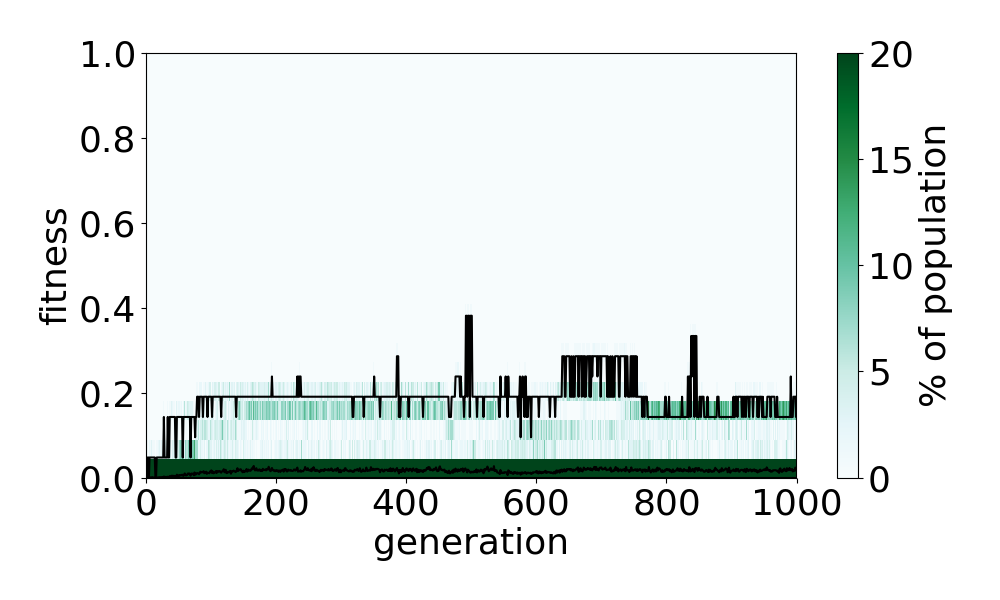
\includegraphics[width=0.3\textwidth]{img/standard_reduced.png} &
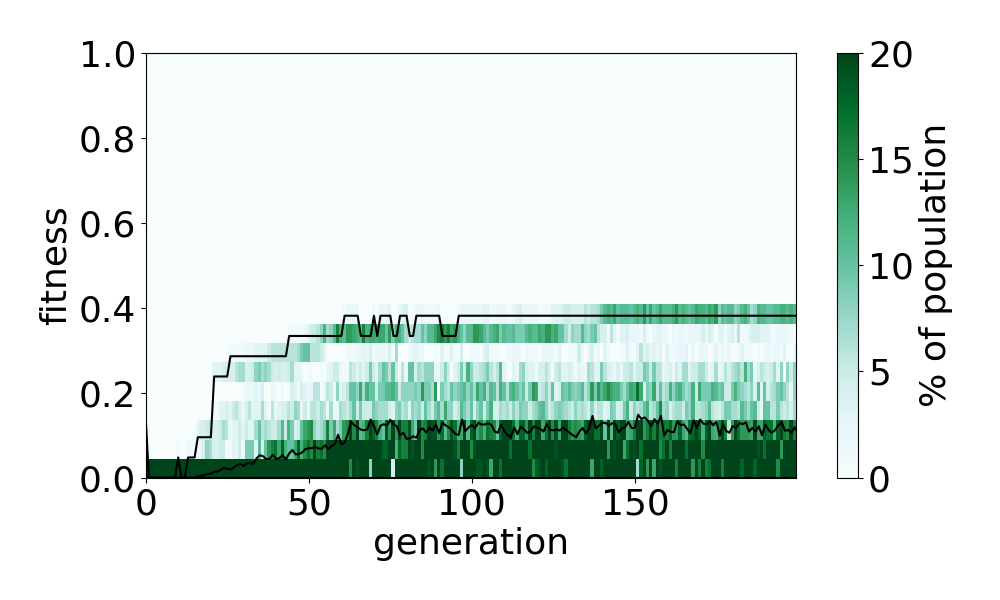
\includegraphics[width=0.3\textwidth]{img/standard_com_11.png} &
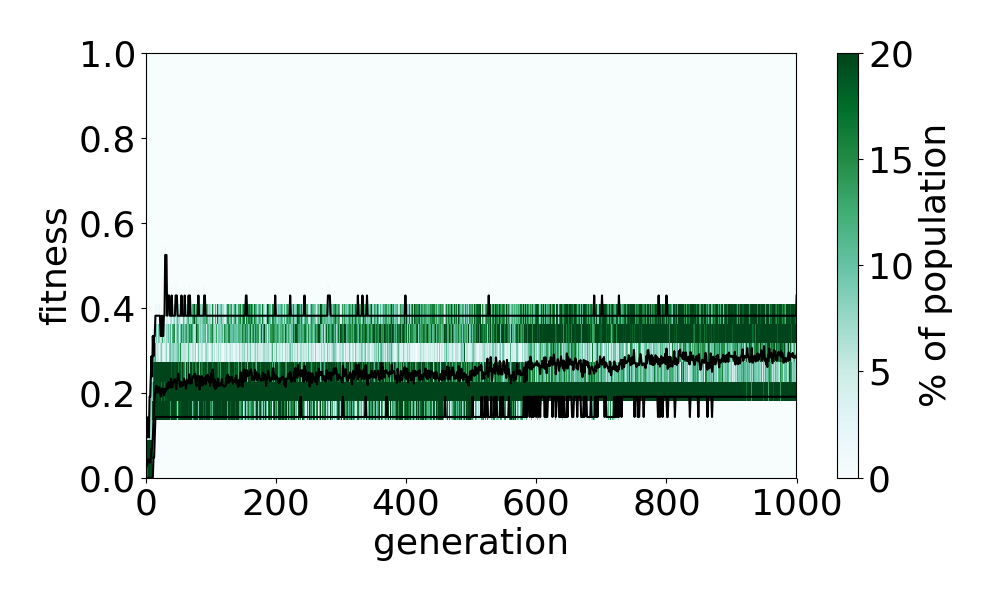
\includegraphics[width=0.3\textwidth]{img/standard_gintonicV9.png} \\
\texttt{hyp014} & \texttt{Union} & \texttt{trainer} \\
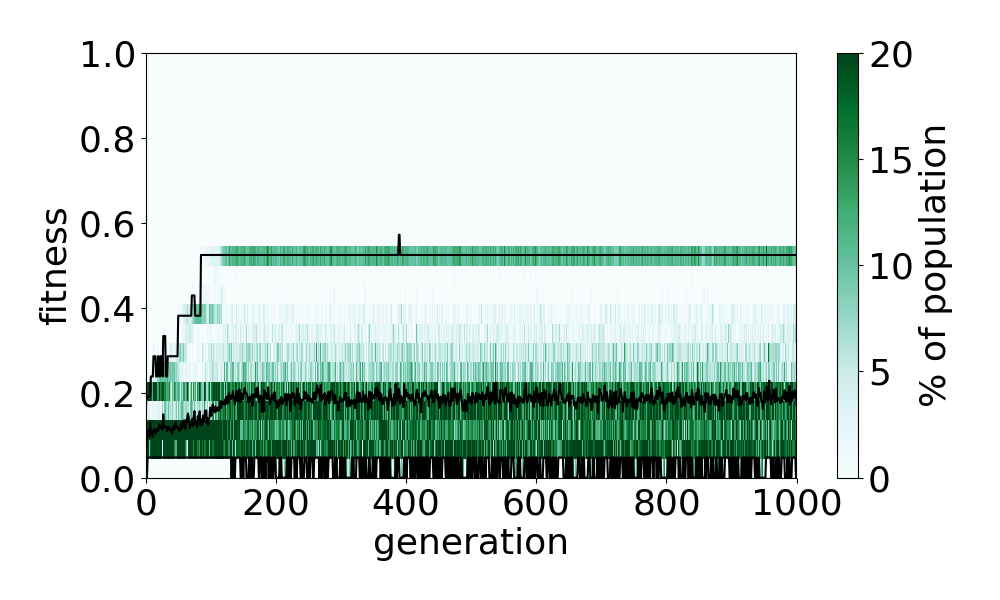
\includegraphics[width=0.3\textwidth]{img/standard_hyp014.png} &
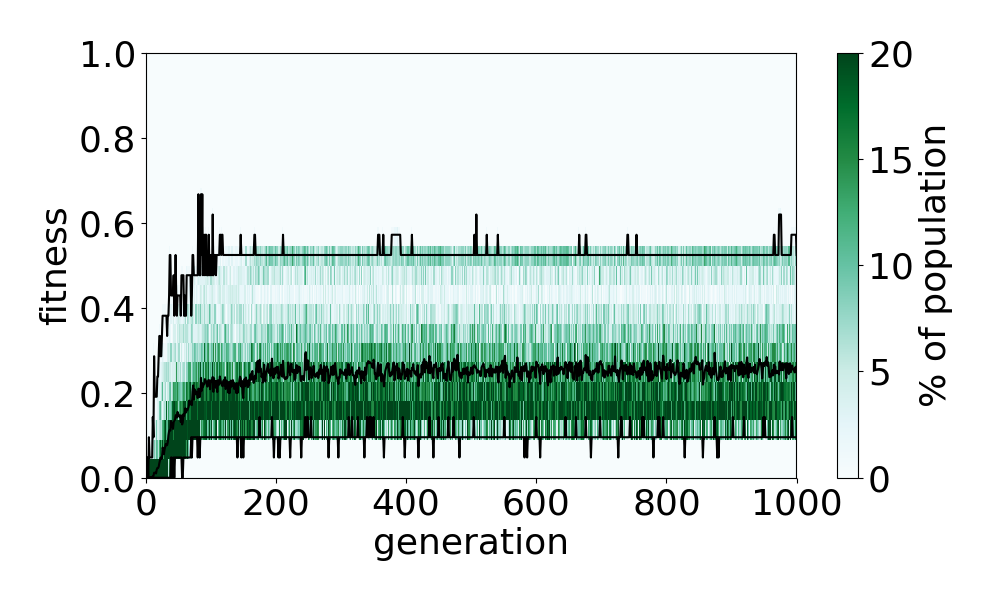
\includegraphics[width=0.3\textwidth]{img/standard_Union.png} &
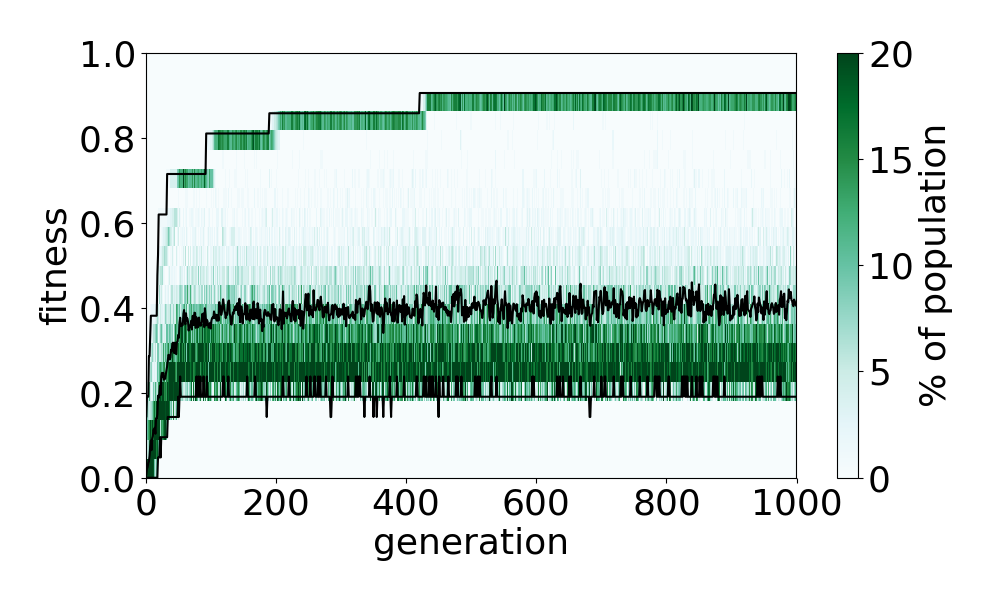
\includegraphics[width=0.3\textwidth]{img/standard_trainer.png}
\end{tabular}
\caption{Fitness density with indicated minimum, average and maximum while training against different bots.}
\label{fig:standard}
\end{figure}

\begin{figure}[H]
\center
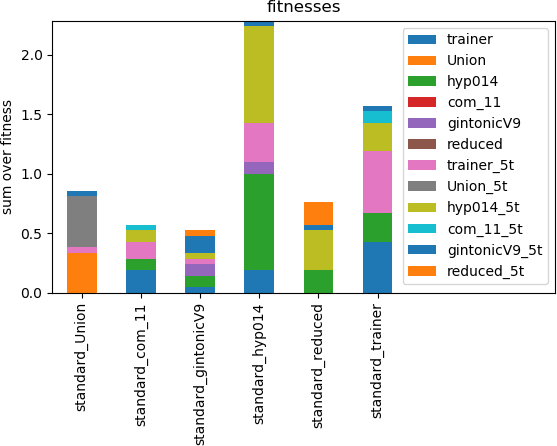
\includegraphics[width=0.4\textwidth]{img/standard.png}
\caption{Cumulative sum of the trained neural networks against all the bots.}
\label{fig:standard_c}
\end{figure}

We can see that the algorithm achieves reasonable scores against the two easiest opponents, \texttt{trainer} and \texttt{hyp014}. Since we were not able to get significantly better results by hyperparameter-tweaking, we theorized that the discrepancy might come from the trainers being too hard to beat by any initial network mutation, providing the same zero fitness for any single useful mutation. Therefore we introduced a weaker, "benevolent" set of trainers that give up after scoring five points by not returning the ball anymore. This lets a specimen that can pass initial serves back receive a positive fitness score. These bots are marked by appending the \texttt{\_5t} suffix to their name.

\begin{figure}[H]
\center
\begin{tabular}{ccc}
\texttt{reduced\_5t} & \texttt{com\_11\_5t} & \texttt{gintonicV9\_5t} \\
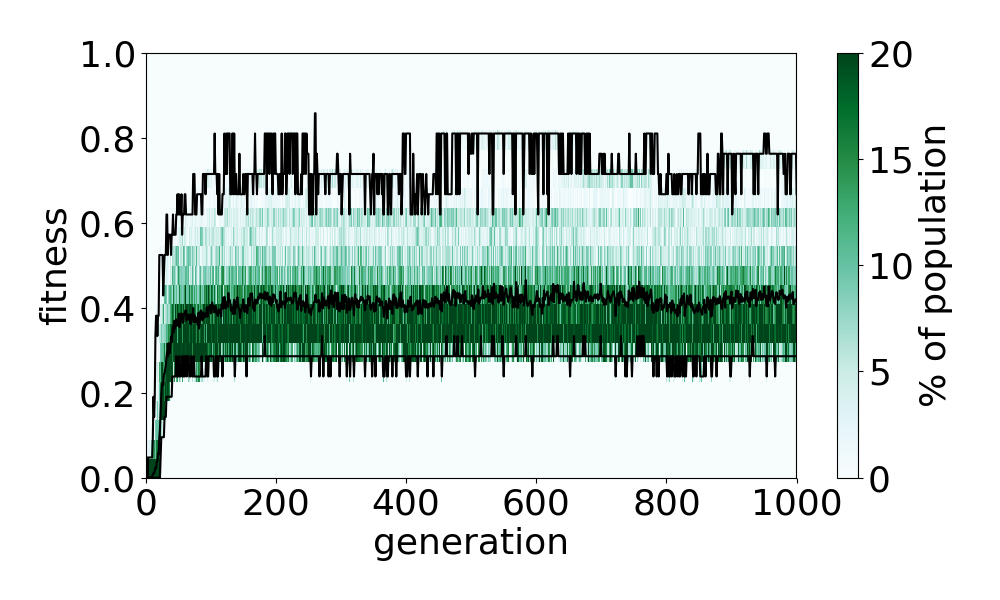
\includegraphics[width=0.3\textwidth]{img/standard_reduced_5t.png} &
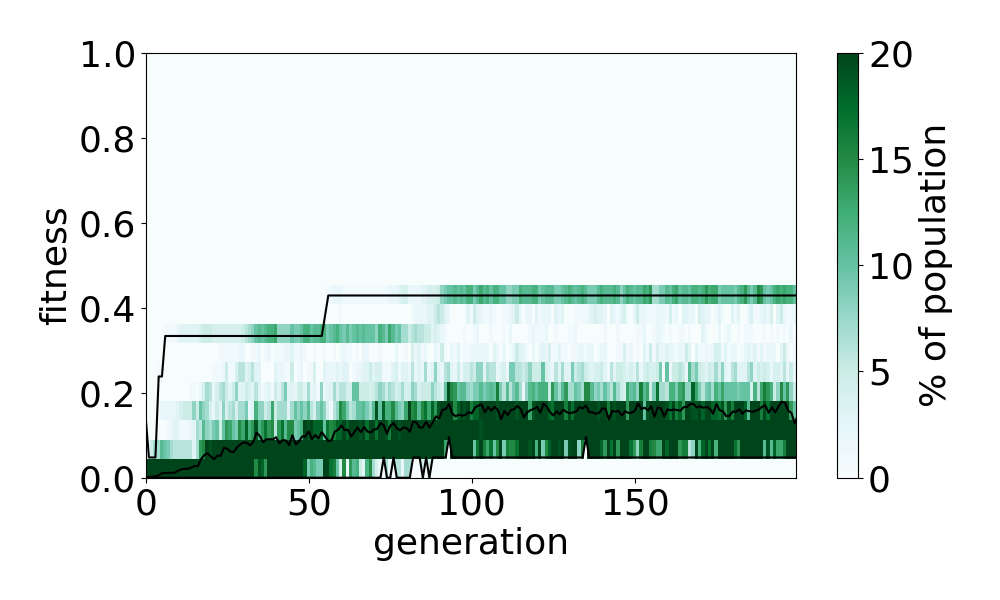
\includegraphics[width=0.3\textwidth]{img/standard_com_11_5t.png} &
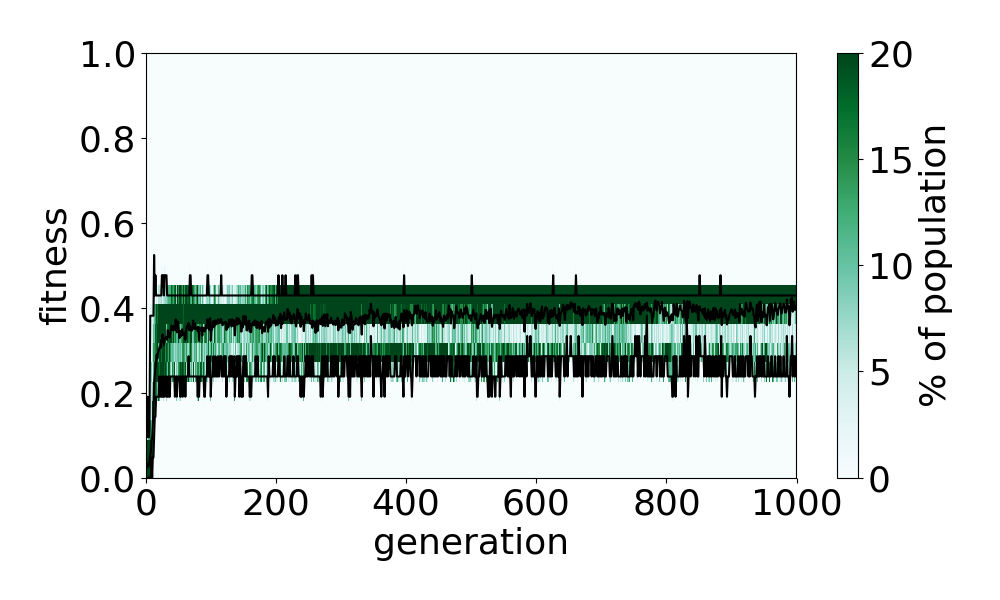
\includegraphics[width=0.3\textwidth]{img/standard_gintonicV9_5t.png} \\
\texttt{hyp014\_5t} & \texttt{Union\_5t} & \texttt{trainer\_5t} \\
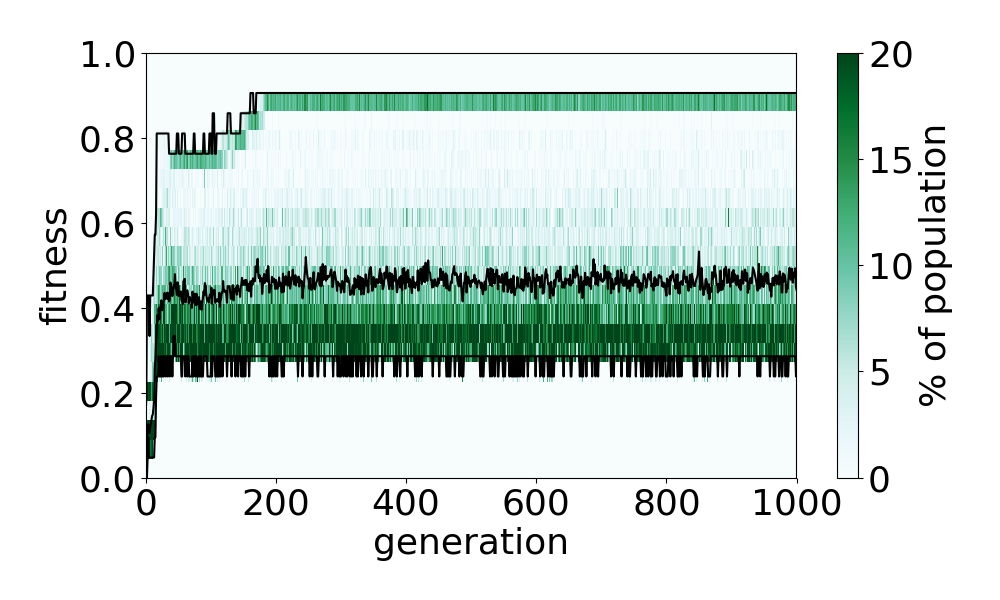
\includegraphics[width=0.3\textwidth]{img/standard_hyp014_5t.png} &
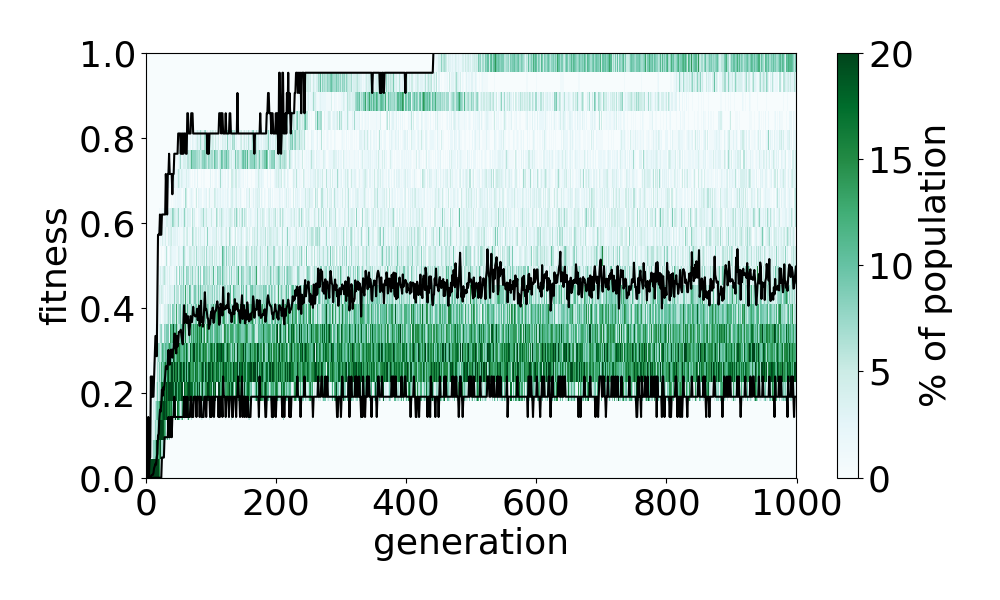
\includegraphics[width=0.3\textwidth]{img/standard_Union_5t.png} &
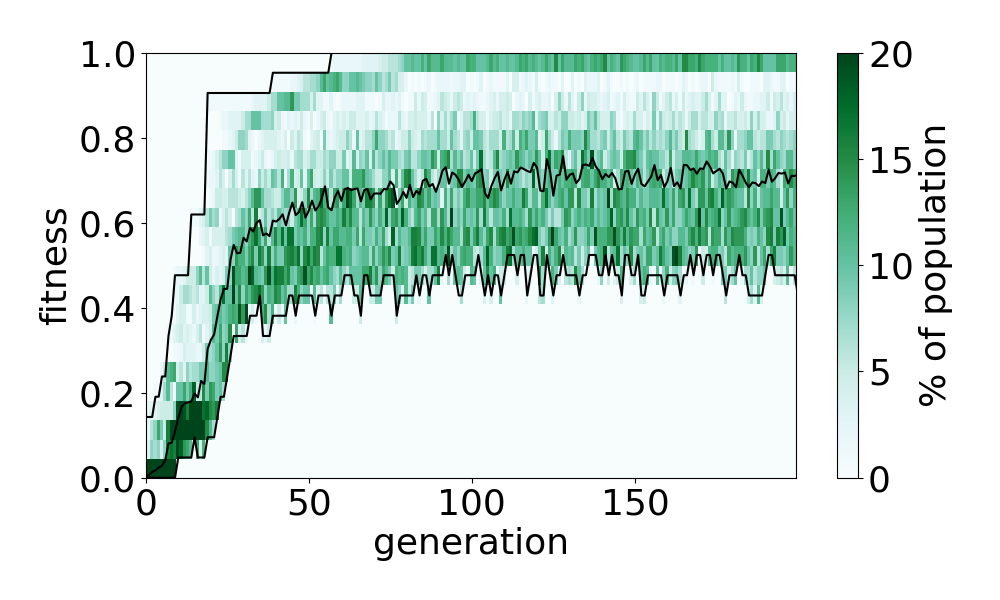
\includegraphics[width=0.3\textwidth]{img/standard_trainer_5t.png}
\end{tabular}
\caption{Fitness density with indicated minimum, average and maximum.}
\label{fig:standard_5t}
\end{figure}

\begin{figure}[H]
\center
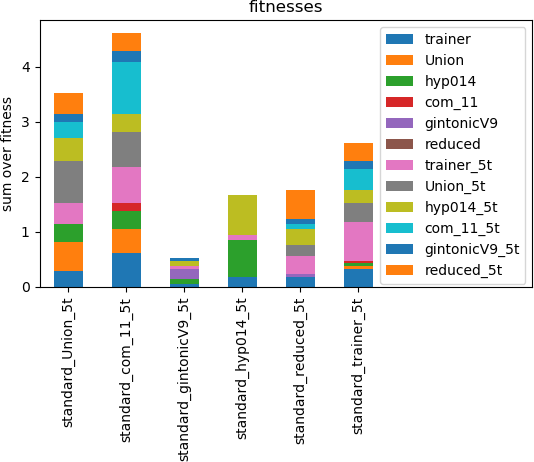
\includegraphics[width=0.4\textwidth]{img/standard_5t.png}
\caption{Best individuals against all bots.}
\label{fig:standard_5t_aa}
\end{figure}

As Fig. \ref{fig:standard_5t} and \ref{fig:standard_5t_aa} show, the networks evolved against the benevolent trainers give significantly better performance against the whole batch of bots, reaching twice the maximum cumulative score.

\section{Per-individual self adaptation}
\label{sec:perind}

\todo{overall: not very pretty graphs <<-- Why do we decided to do self adaptation?}

We first implemented a method similar to (1) and (4) from \cite{self_adapt}, giving each individual a mutation rate and a sigma value. These were mutated when the individual was selected for mutation. Their initialization was also random, in the range of [0.25, 0.75] for the mutation rate and [0, 0.03] for the sigma values.

\subsection{Numerical tests}

\begin{figure}[H]
\center
\begin{tabular}{ccc}
\texttt{reduced} & \texttt{com\_11} & \texttt{gintonicV9} \\
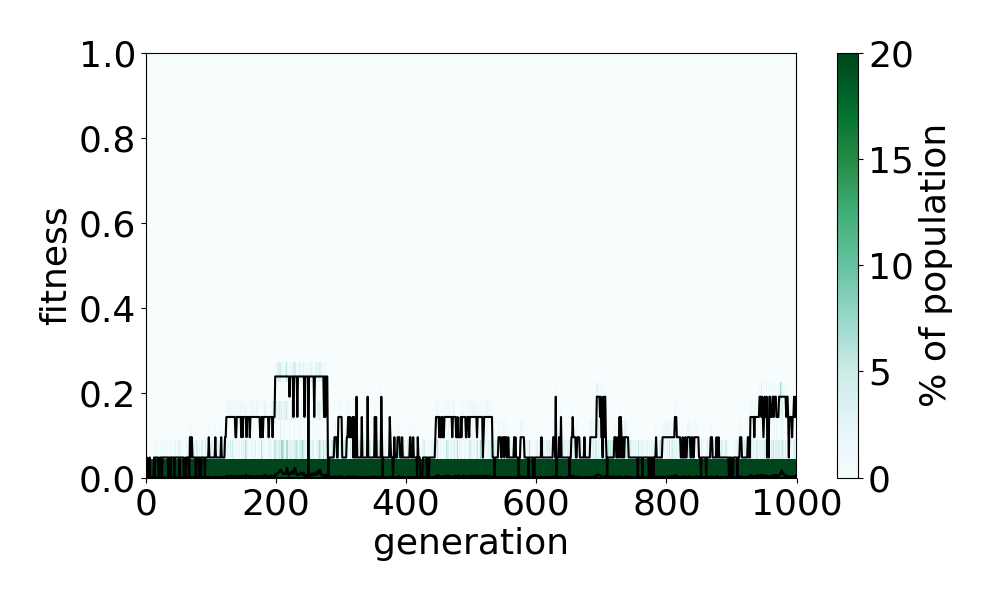
\includegraphics[width=0.3\textwidth]{img/self_adapt_1_reduced.png} &
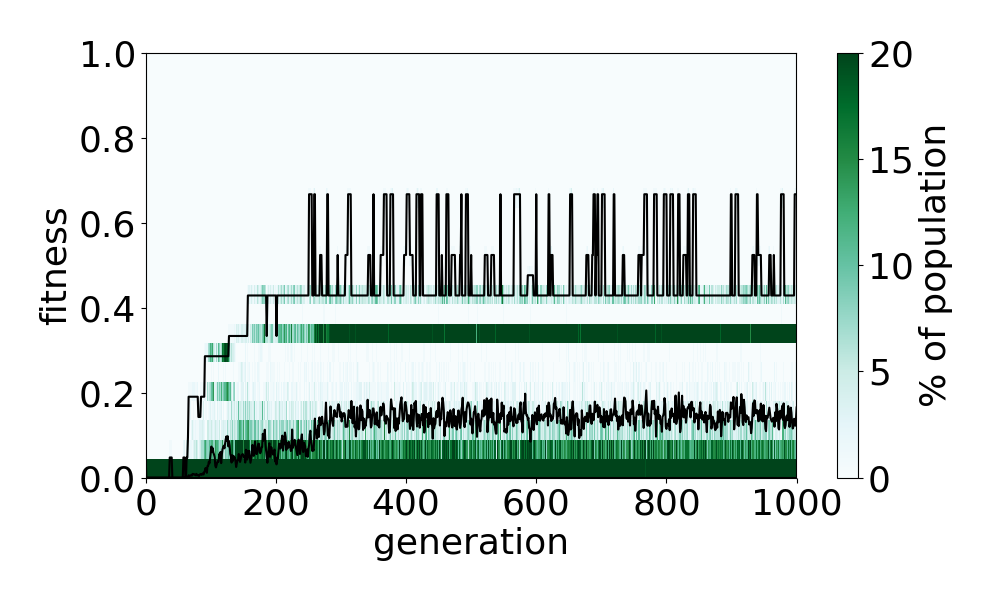
\includegraphics[width=0.3\textwidth]{img/self_adapt_1_com_11.png} &
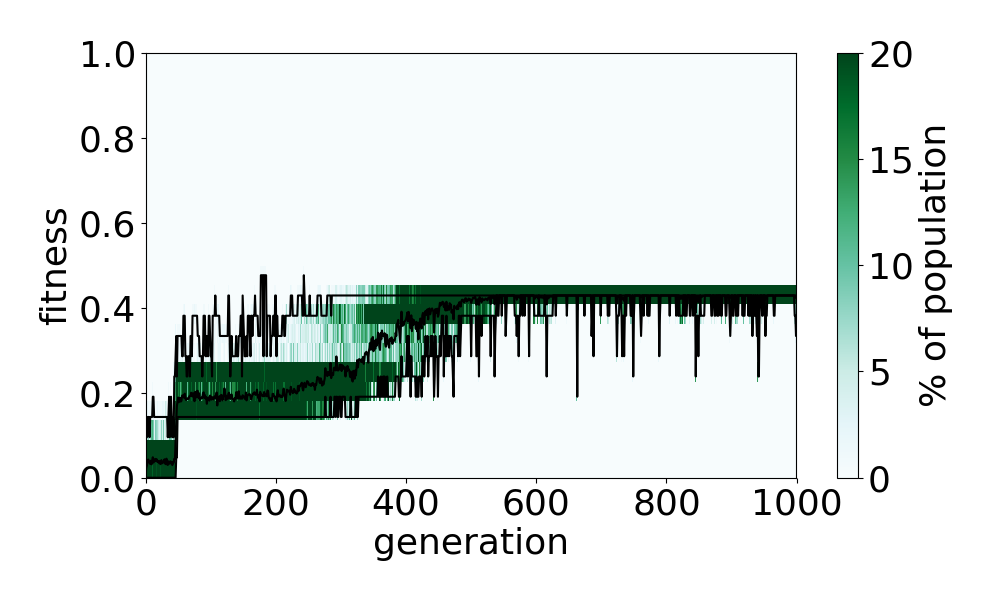
\includegraphics[width=0.3\textwidth]{img/self_adapt_1_gintonicV9.png} \\
\texttt{hyp014} & \texttt{Union} & \texttt{trainer} \\
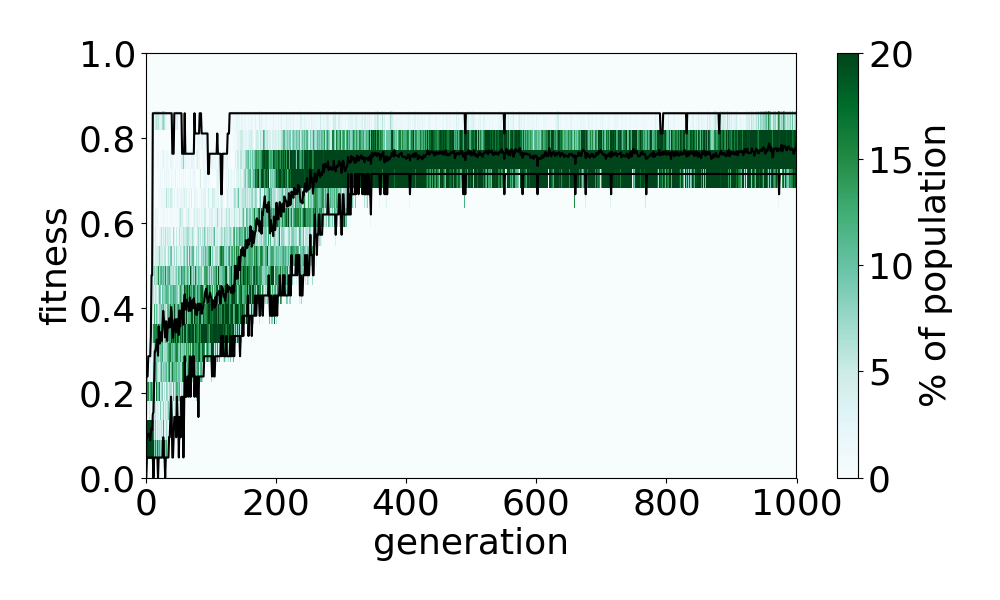
\includegraphics[width=0.3\textwidth]{img/self_adapt_1_hyp014.png} &
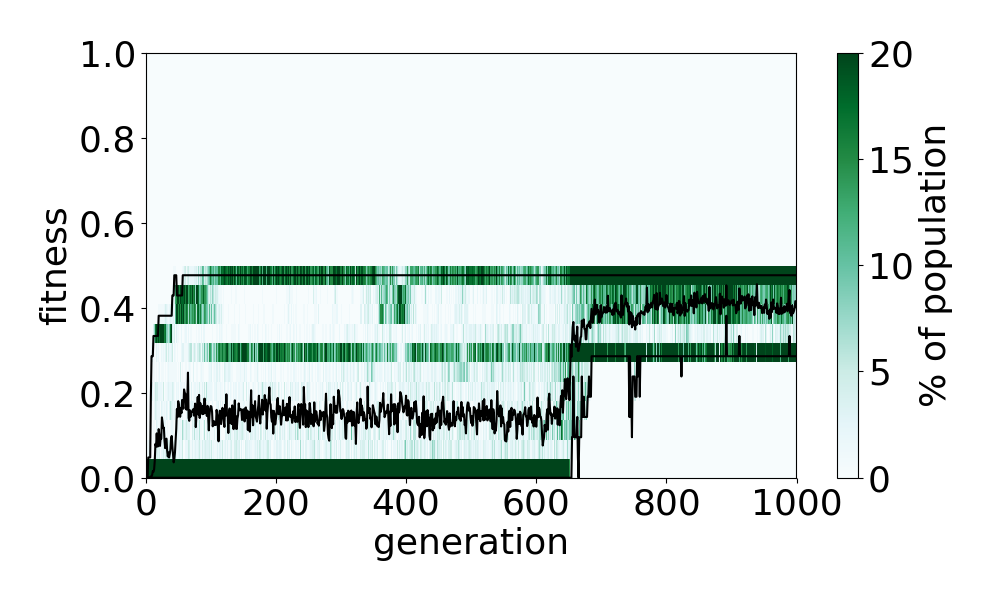
\includegraphics[width=0.3\textwidth]{img/self_adapt_1_Union.png} &
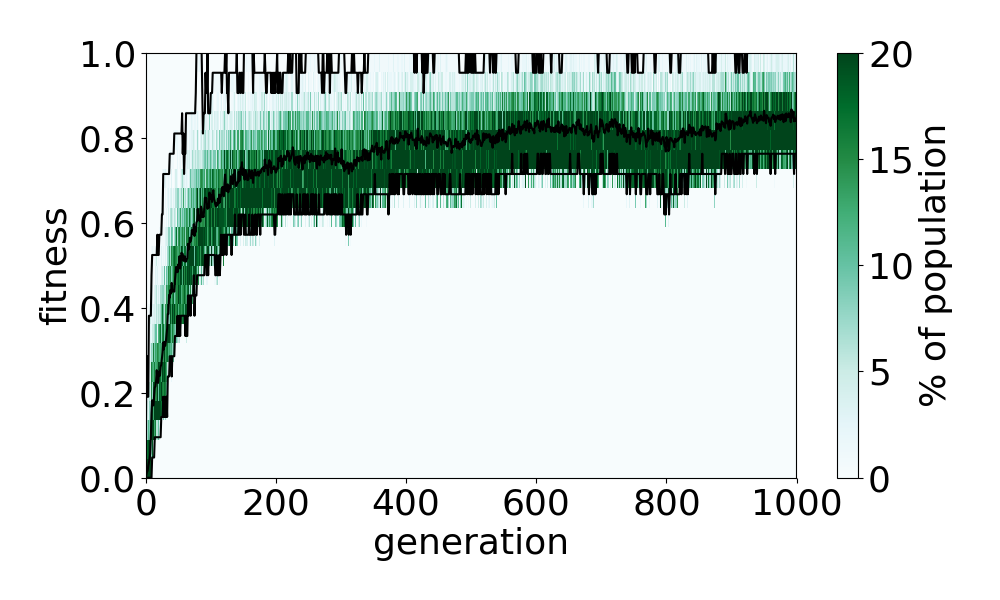
\includegraphics[width=0.3\textwidth]{img/self_adapt_1_trainer.png}
\end{tabular}
\caption{Fitness density with indicated minimum, average and maximum.}
\label{fig:self_adapt_1}
\end{figure}

\begin{figure}[H]
\center
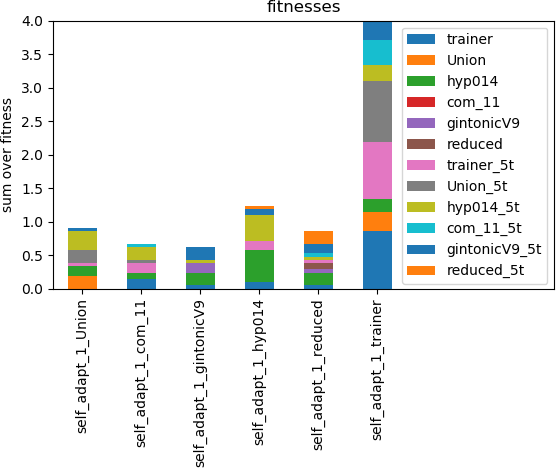
\includegraphics[width=0.4\textwidth]{img/self_adapt_1.png}
\caption{Best individuals against all bots.}
\label{fig:self_adapt_1_aa}
\end{figure}

\begin{figure}[H]
\center
\begin{tabular}{ccc}
\texttt{reduced\_5t} & \texttt{com\_11\_5t} & \texttt{gintonicV9\_5t} \\
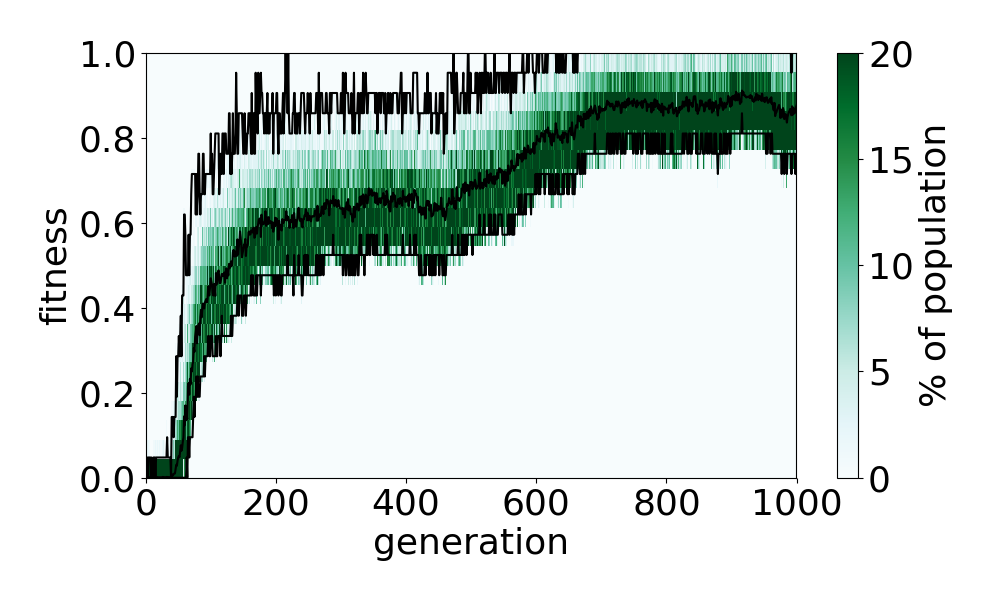
\includegraphics[width=0.3\textwidth]{img/self_adapt_1_reduced_5t.png} &
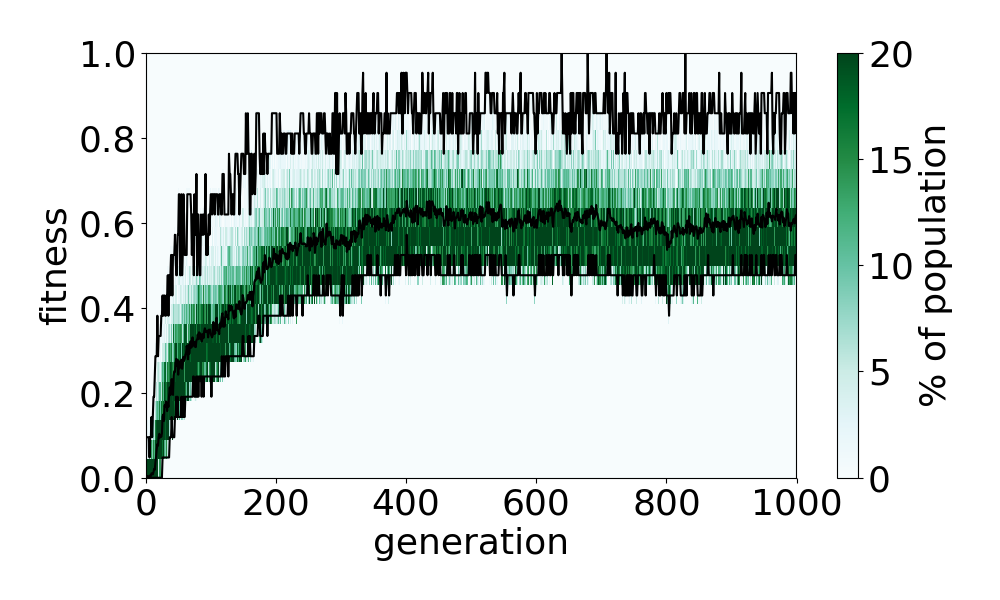
\includegraphics[width=0.3\textwidth]{img/self_adapt_1_com_11_5t.png} &
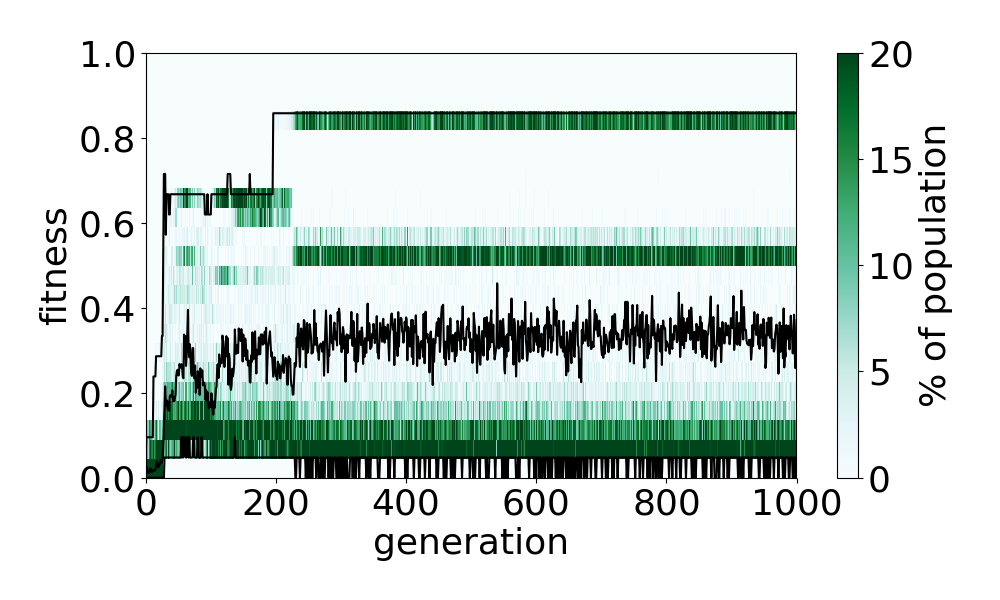
\includegraphics[width=0.3\textwidth]{img/self_adapt_1_gintonicV9_5t.png} \\
\texttt{hyp014\_5t} & \texttt{Union\_5t} & \texttt{trainer\_5t} \\
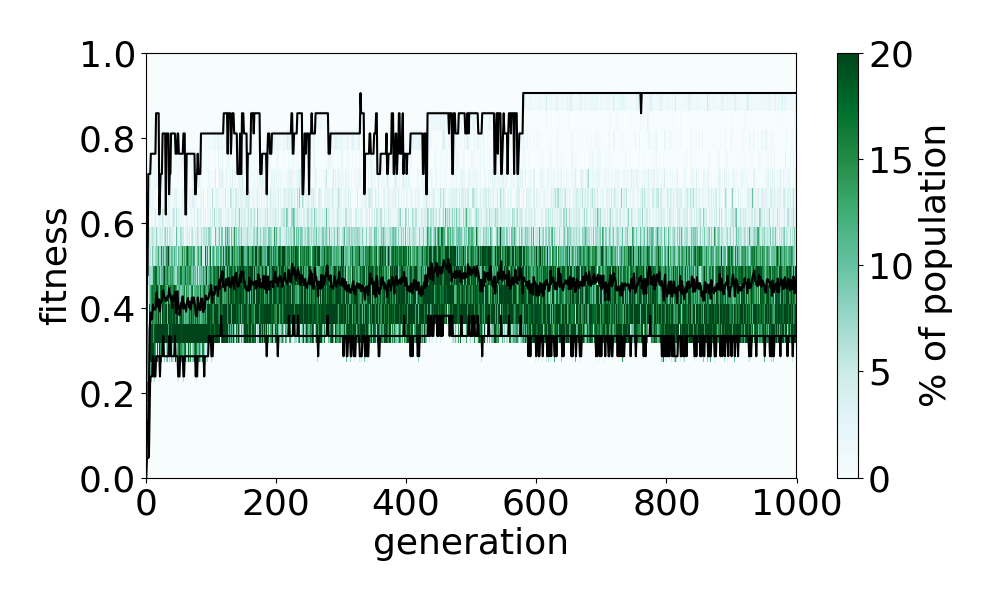
\includegraphics[width=0.3\textwidth]{img/self_adapt_1_hyp014_5t.png} &
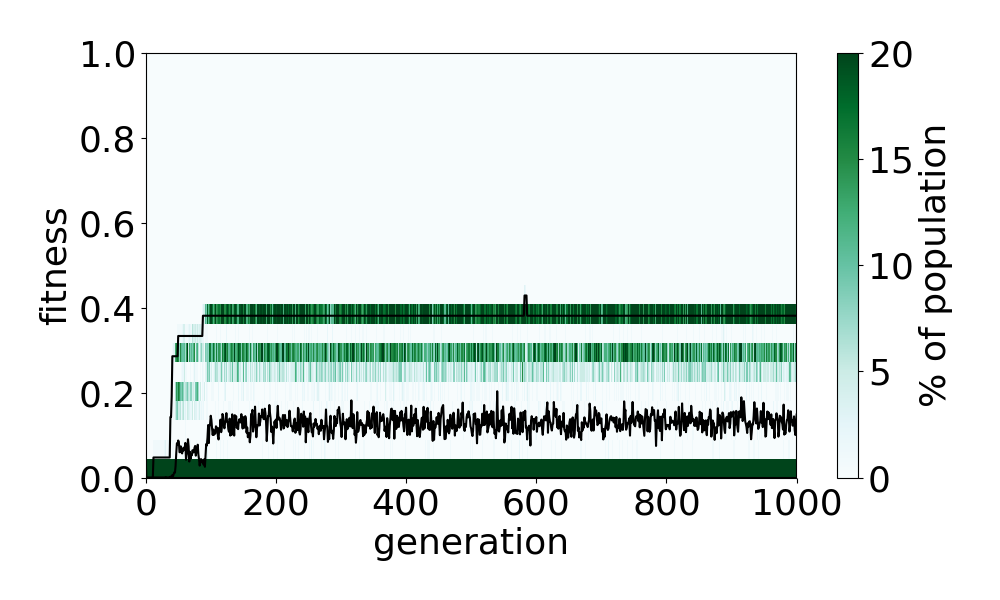
\includegraphics[width=0.3\textwidth]{img/self_adapt_1_Union_5t.png} &
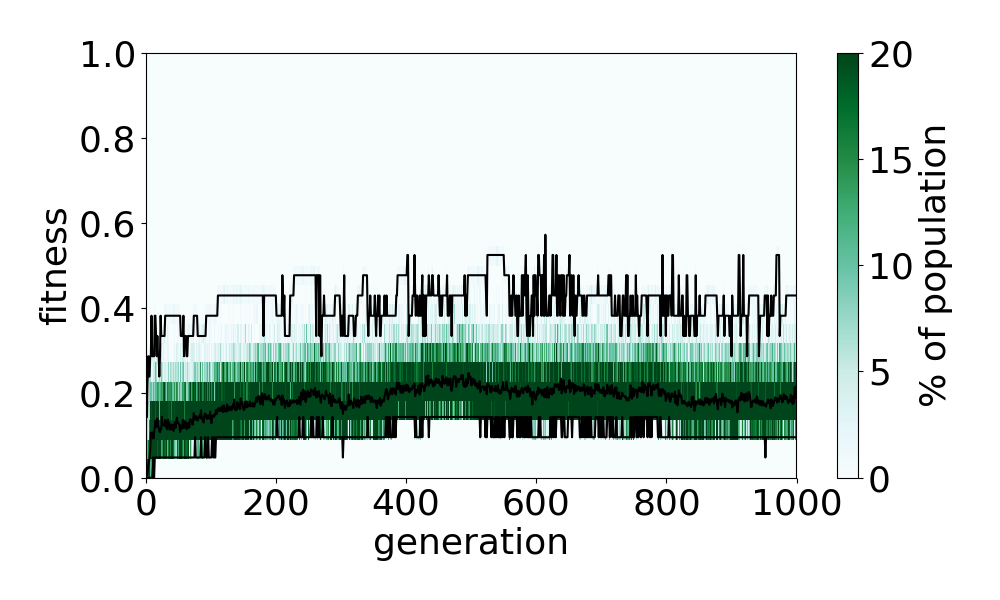
\includegraphics[width=0.3\textwidth]{img/self_adapt_1_trainer_5t.png}
\end{tabular}
\caption{Fitness density with indicated minimum, average and maximum.}
\label{fig:self_adapt_1_5t}
\end{figure}

\begin{figure}[H]
\center
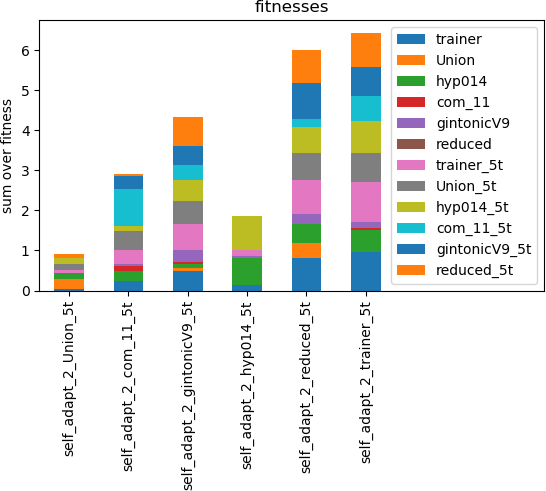
\includegraphics[width=0.4\textwidth]{img/self_adapt_2_5t.png}
\caption{Best individuals against all bots.}
\label{fig:self_adapt_1_5t_aa}
\end{figure}

We can see in figures \ref{fig:self_adapt_1_5t} and \ref{fig:self_adapt_1_5t_aa} that the results improve significantly in both cases. Self adaptation causes the networks trained on \texttt{\_5t} opponents to get consistent results across the board.

The surprisingly low performance against the easiest bot, \texttt{trainer\_5t} might be explained by the bot being too easy. The high initial fitness might encourage the survival of individuals with a low mutation rate, causing the algorithm to get stuck in a local optimum.

\todo{trainer5t does not coincide on the two graphs, what happened? We get a good result against trainer5t according to the bottom graph}

\section{Per-parameter self adaptation}

We also explored a method similar to (2) and (5) in \cite{self_adapt}, where each parameter gets it's own mutation sigma parameter. This produces similar results to per-individual self adaptation with harsh teachers, but with benevolent teachers fails to reproduce the consistency of the other method.

\subsection{Numerical tests}

\begin{figure}[H]
\center
\begin{tabular}{ccc}
\texttt{reduced} & \texttt{com\_11} & \texttt{gintonicV9} \\
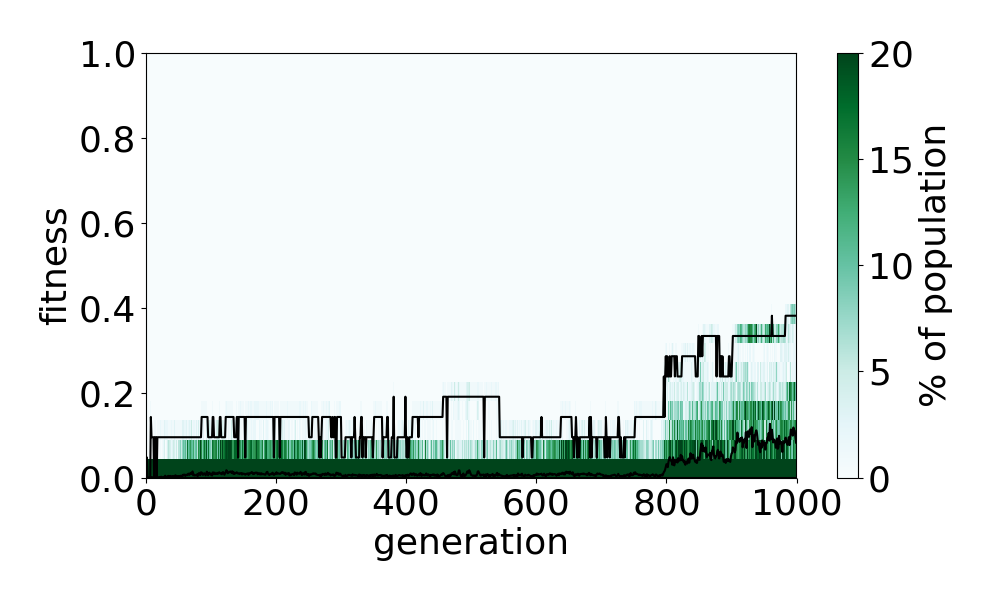
\includegraphics[width=0.3\textwidth]{img/self_adapt_2_reduced.png} &
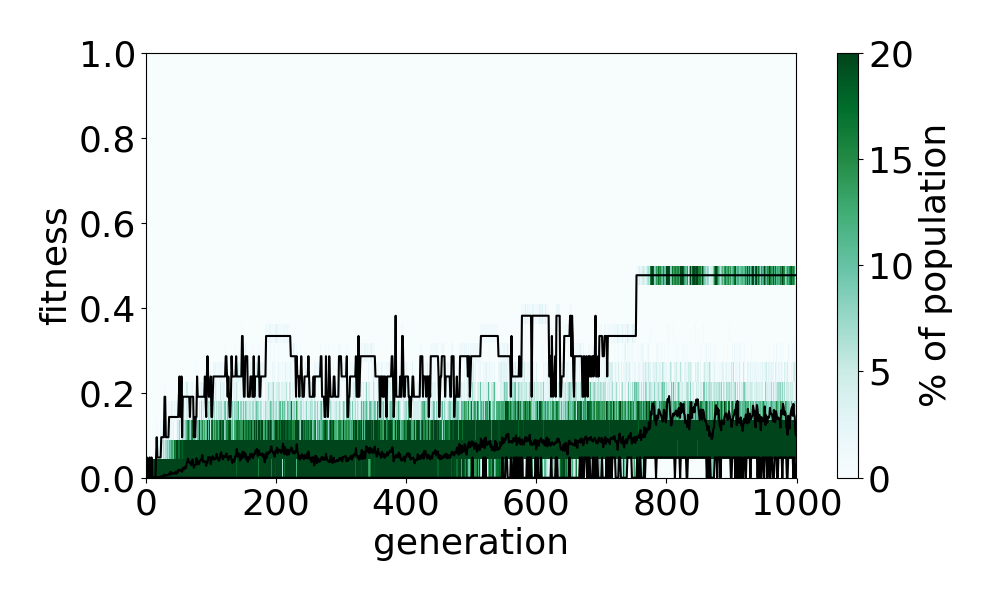
\includegraphics[width=0.3\textwidth]{img/self_adapt_2_com_11.png} &
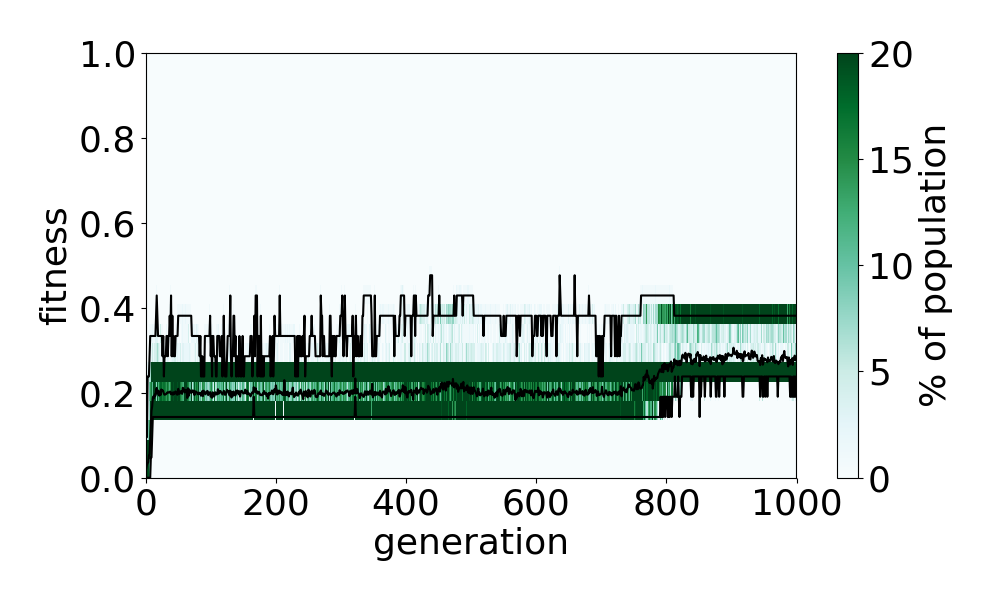
\includegraphics[width=0.3\textwidth]{img/self_adapt_2_gintonicV9.png} \\
\texttt{hyp014} & \texttt{Union} & \texttt{trainer} \\
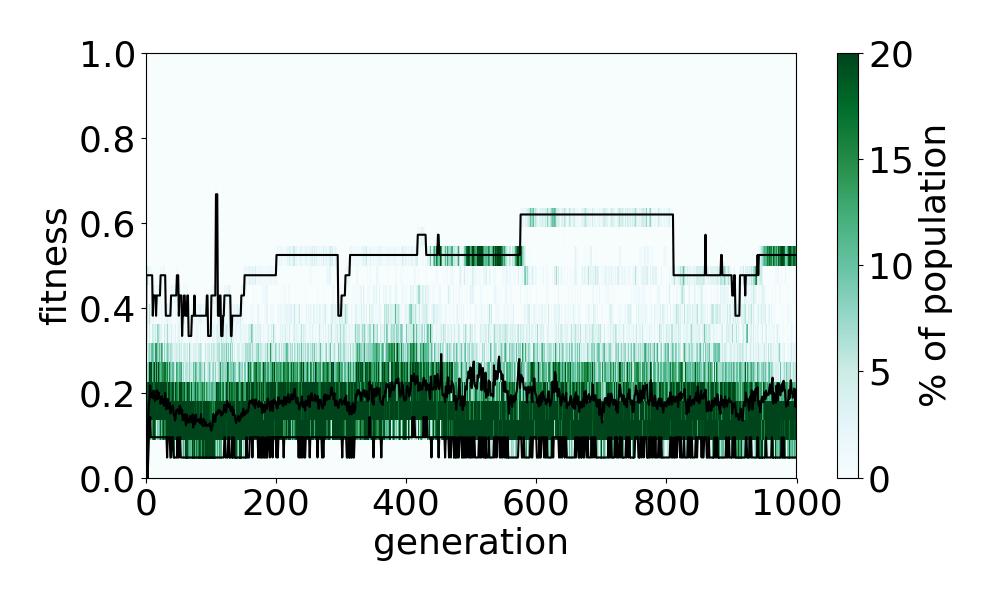
\includegraphics[width=0.3\textwidth]{img/self_adapt_2_hyp014.png} &
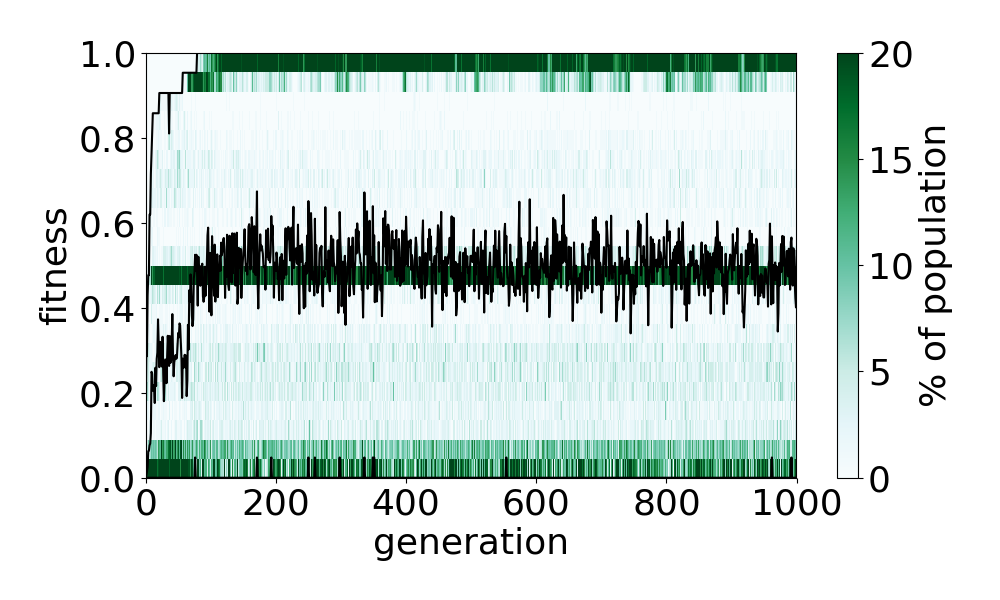
\includegraphics[width=0.3\textwidth]{img/self_adapt_2_Union.png} &
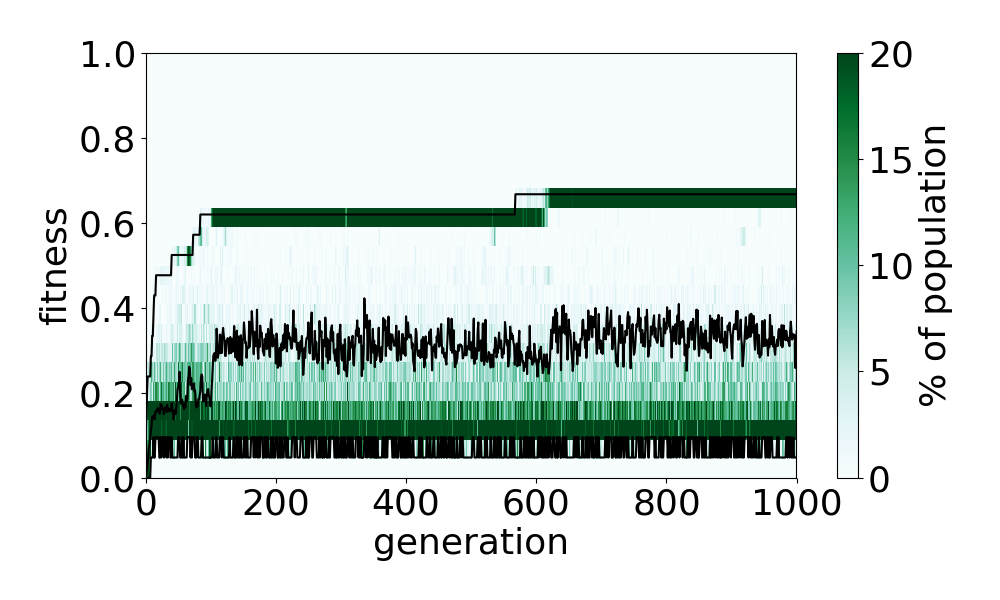
\includegraphics[width=0.3\textwidth]{img/self_adapt_2_trainer.png}
\end{tabular}
\caption{Fitness density with indicated minimum, average and maximum.}
\label{fig:self_adapt_2}
\end{figure}

\begin{figure}[H]
\center
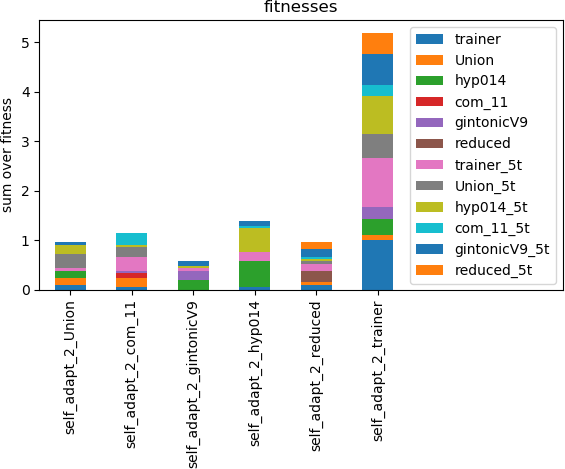
\includegraphics[width=0.4\textwidth]{img/self_adapt_2.png}
\caption{Best individuals against all bots.}
\label{fig:self_adapt_2_aa}
\end{figure}

\begin{figure}[H]
\center
\begin{tabular}{ccc}
\texttt{reduced\_5t} & \texttt{com\_11\_5t} & \texttt{gintonicV9\_5t} \\
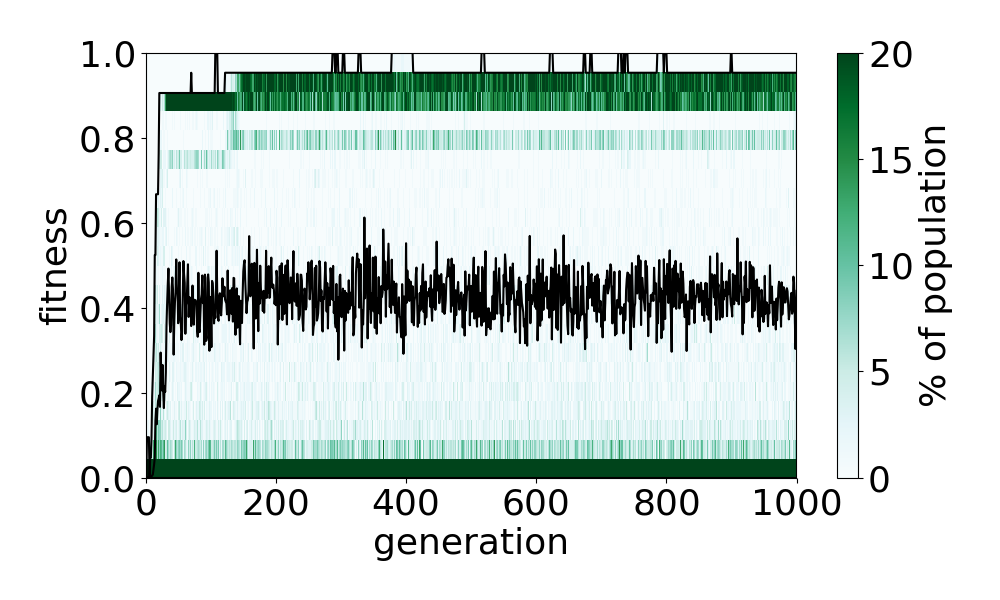
\includegraphics[width=0.3\textwidth]{img/self_adapt_2_reduced_5t.png} &
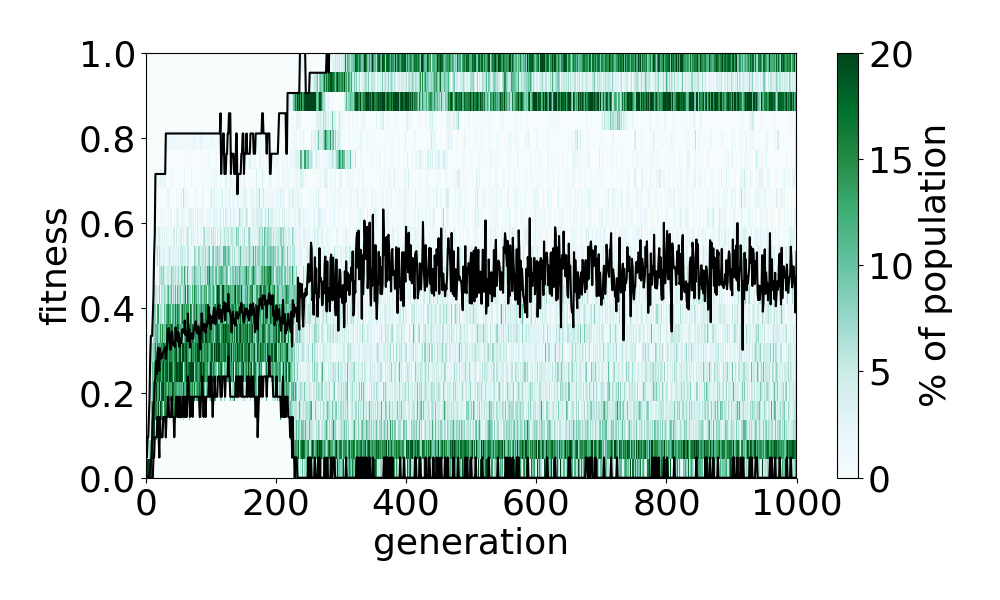
\includegraphics[width=0.3\textwidth]{img/self_adapt_2_com_11_5t.png} &
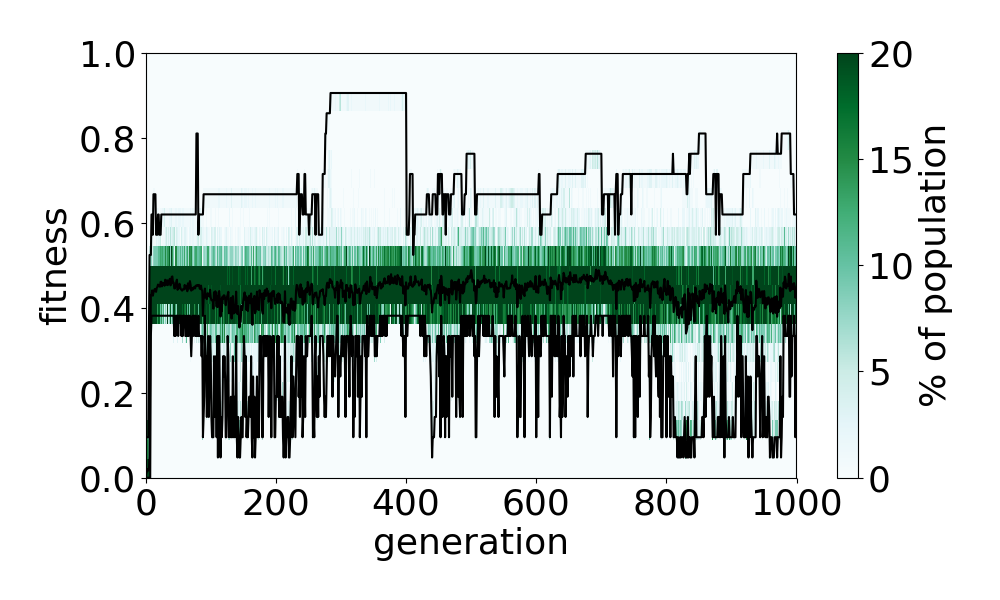
\includegraphics[width=0.3\textwidth]{img/self_adapt_2_gintonicV9_5t.png} \\
\texttt{hyp014\_5t} & \texttt{Union\_5t} & \texttt{trainer\_5t} \\
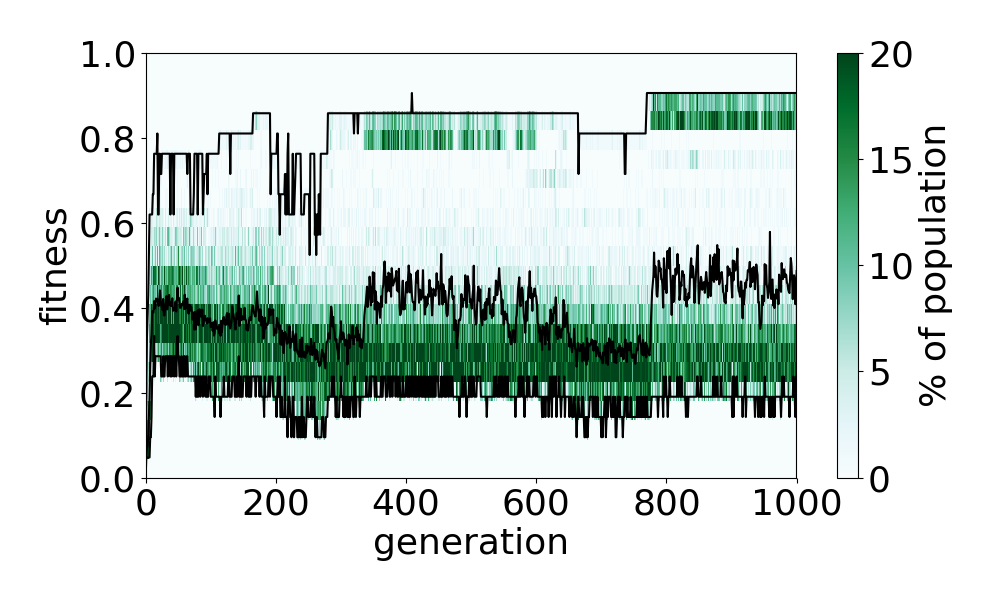
\includegraphics[width=0.3\textwidth]{img/self_adapt_2_hyp014_5t.png} &
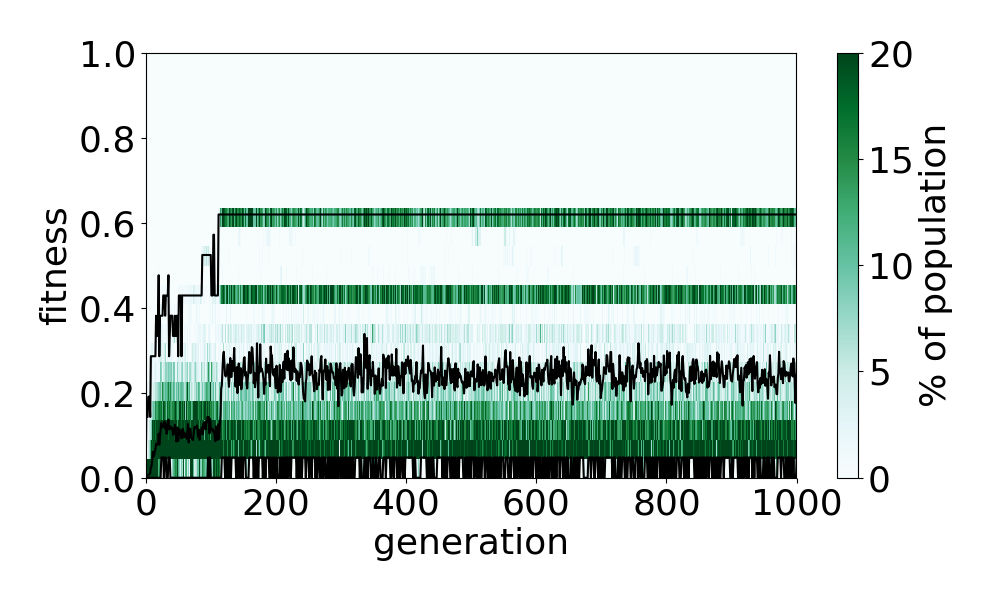
\includegraphics[width=0.3\textwidth]{img/self_adapt_2_Union_5t.png} &
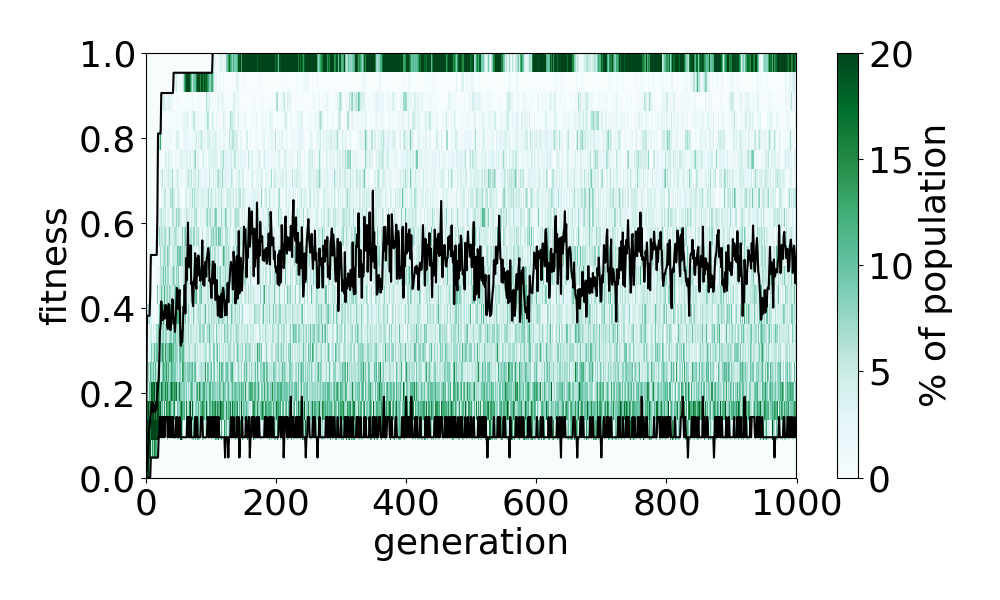
\includegraphics[width=0.3\textwidth]{img/self_adapt_2_trainer_5t.png}
\end{tabular}
\caption{Fitness density with indicated minimum, average and maximum.}
\label{fig:self_adapt_2_5t}
\end{figure}

\begin{figure}[H]
\center
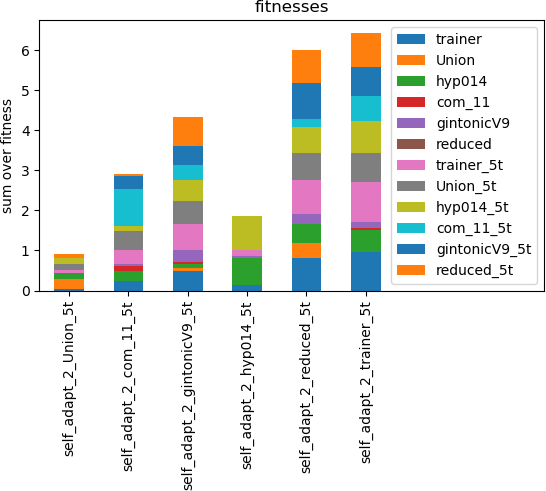
\includegraphics[width=0.4\textwidth]{img/self_adapt_2_5t.png}
\caption{Best individuals against all bots.}
\label{fig:self_adapt_2_5t_aa}
\end{figure}

\section{Curriculum learning}

We implemented a limited set of curriculum learning, where the training happens against increasingly harder opponents \texttt{gintonicV9\_5t}, \texttt{com\_11\_5t}, \texttt{gintonicV9}, and \texttt{com\_11} for 200 generations each. These bots previously worked as solid teachers. As can be seen on \ref{fig:change}, only the Per-individual self adaptation seems to work, there's no transfer of knowledge between the different bots for the other methods.

It's possible that with increasing the number of generations this algorithm would produce some advantages over training with just one teacher, but we couldn't finish the longer experiment due to time constraints.

\begin{figure}[H]
\center
\begin{tabular}{ccc}
standard & per-individual s. a. & per-parameter s. a. \\
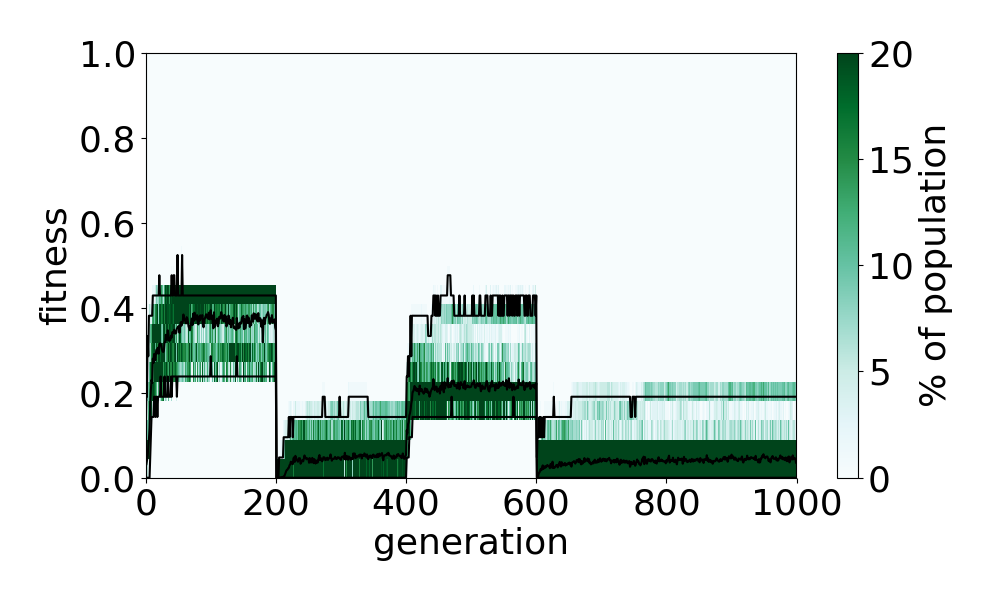
\includegraphics[width=0.3\textwidth]{img/standard_gintonicV9_5t_com_11_5t_gintonicV9_com_11.png} &
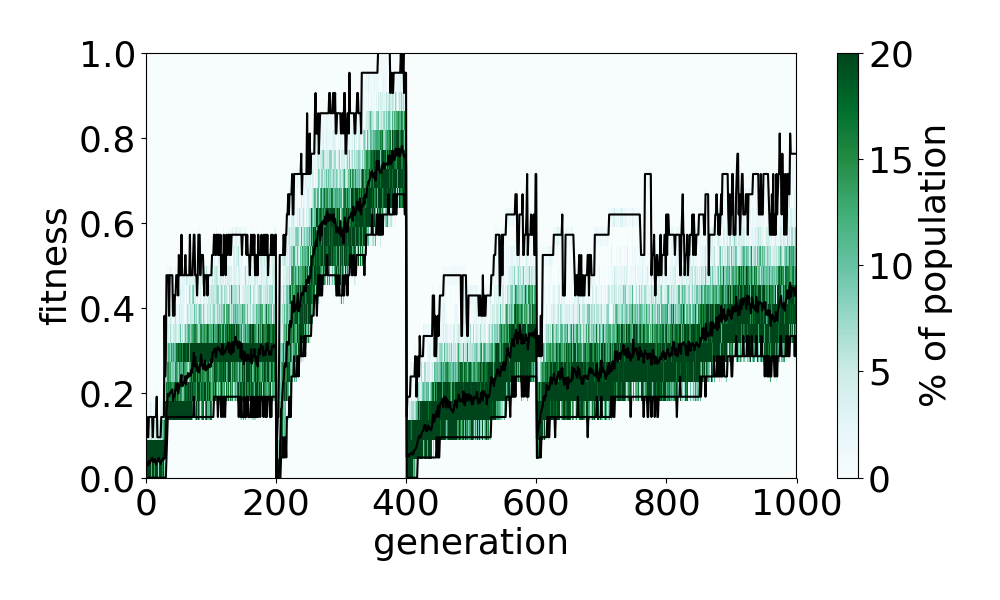
\includegraphics[width=0.3\textwidth]{img/self_adapt_1_gintonicV9_5t_com_11_5t_gintonicV9_com_11.png} &
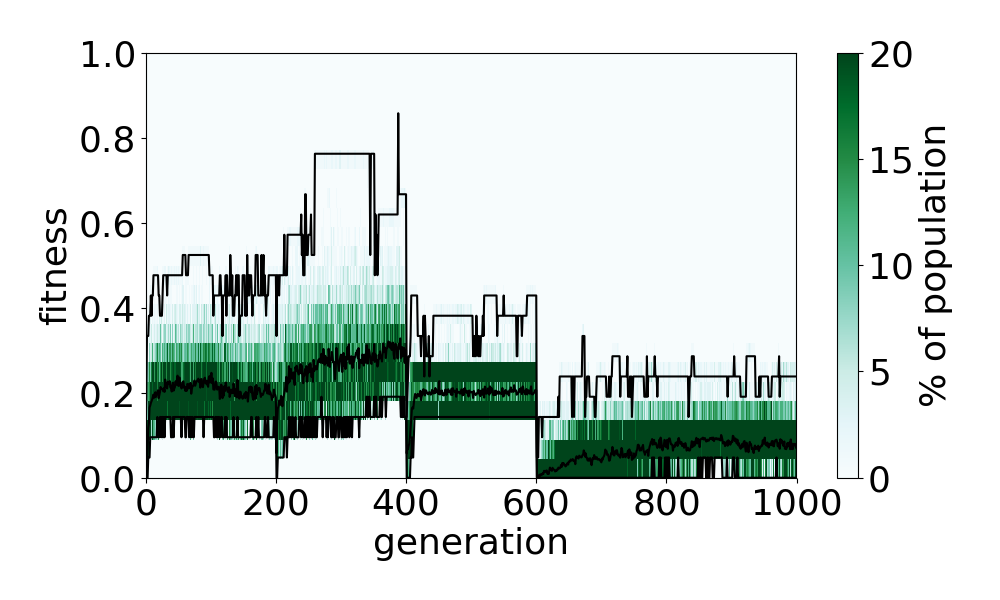
\includegraphics[width=0.3\textwidth]{img/self_adapt_2_gintonicV9_5t_com_11_5t_gintonicV9_com_11.png} \\
\end{tabular}
\caption{Fitness density with indicated minimum, average and maximum.}
\label{fig:changing opponent}
\end{figure}

\begin{figure}[H]
\center
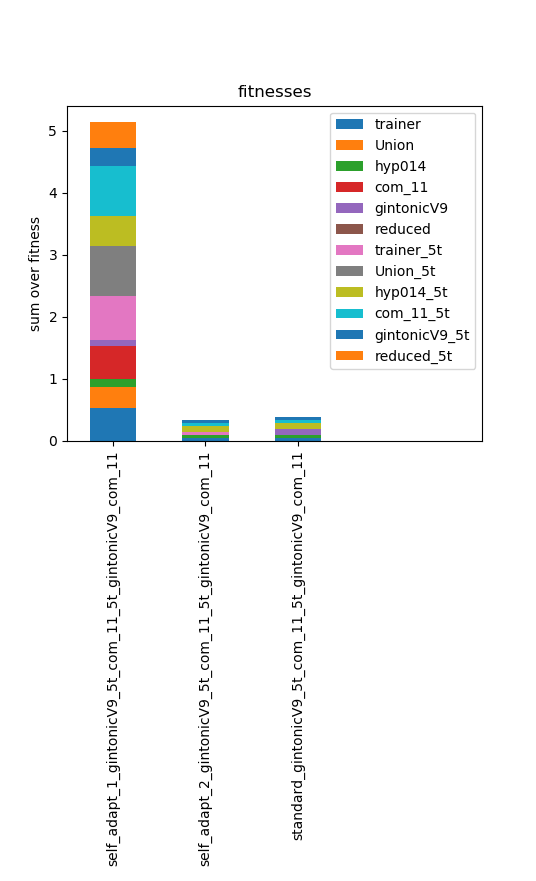
\includegraphics[width=0.4\textwidth]{img/change.png}
\caption{Best individuals against all bots.}
\label{fig:change}
\end{figure}

\section{Self-training}
Implementing self-training based on \cite{Sims94evolving3d}.

\subsection{All vs best}
We ran a version of the algorithm where the fitness function was evaluated on the best specimen of the last generation.

\begin{figure}[H]
\center
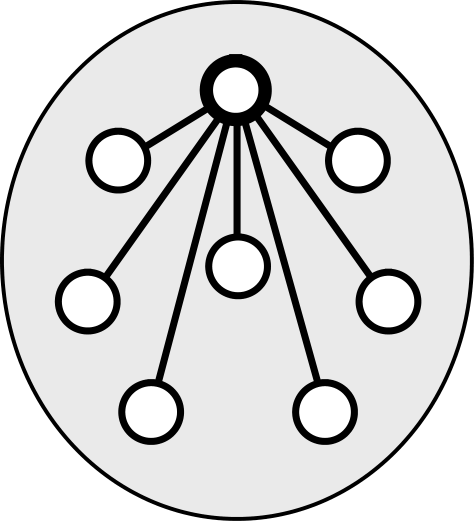
\includegraphics[width=0.155555\textwidth]{img/scheme_self_training_1.png}
\caption{Scheme for all vs best training; source: \cite{Sims94evolving3d}.}
\label{fig:scheme_self_training_1}
\end{figure}

\begin{figure}[H]
\center
\begin{tabular}{cc}
standard & self adapt 1\\
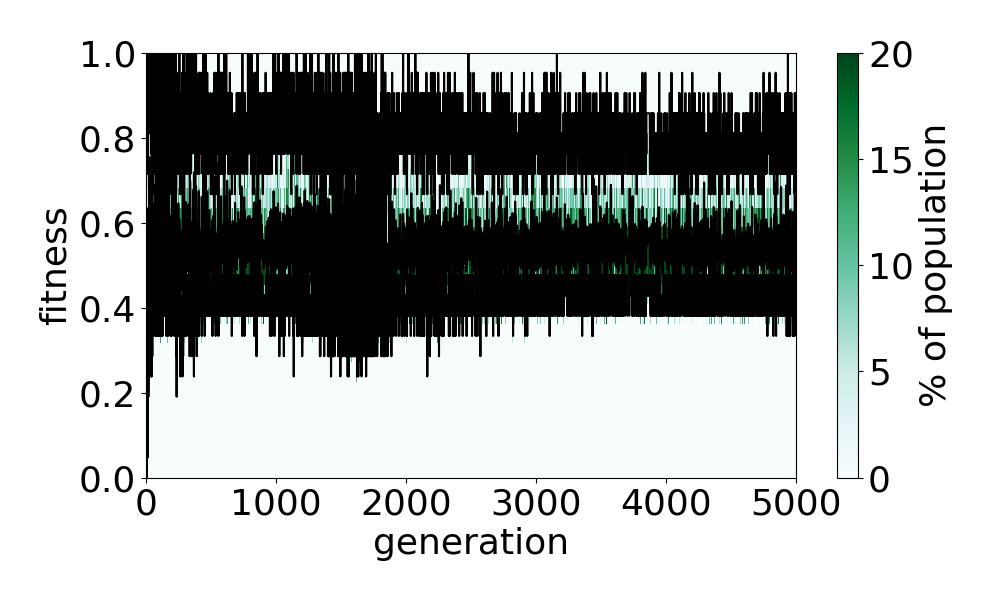
\includegraphics[width=0.3\textwidth]{img/standard_last_best.png} &
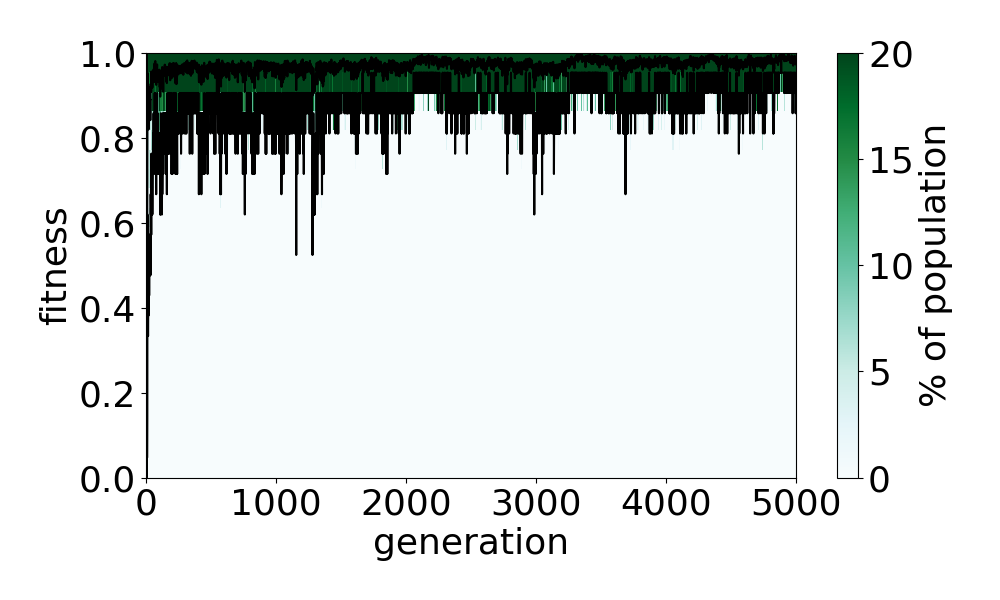
\includegraphics[width=0.3\textwidth]{img/self_adapt_1_last_best.png}
\end{tabular}
\caption{Fitness density with indicated minimum, average and maximum.}
\label{fig:last_best}
\end{figure}

\begin{figure}[H]
\center
\includegraphics[width=0.3\textwidth]{img/self_training_1.png}
\caption{Best individuals against all bots.}
\label{fig:self_training_1}
\end{figure}

Since we start out with evaluating against easy opponents, it's a possibility for the algorithm to get stuck in a local optimum like it did with per-individual self adaptation. While the standard method works nice, (see figures \ref{fig:last_best} and \ref{fig:self_training_1}) the self-adaption variant fails to produce any meaningful result despite the high fitness value, thus supporting our theory from section \ref{sec:perind}.

\subsection{Two-species all vs best}

This implementation of the idea from \cite{Sims94evolving3d} uses two species (named left and right, after the side they played on in-game) that are always evaluated against the other. The population size was 100 for each of the species.

\begin{figure}[H]
\center
\includegraphics[width=0.155555\textwidth]{img/scheme_self_training_2.png}
\caption{Scheme for two-species all vs best self training; source: \cite{Sims94evolving3d}.}
\label{fig:scheme_self_training_2}
\end{figure}

\begin{figure}[H]
\center
\begin{tabular}{cc}
standard left side & standard right side \\
\includegraphics[width=0.3\textwidth]{img/standard_self_training_2_1.png} &
\includegraphics[width=0.3\textwidth]{img/standard_self_training_2_2.png} \\
self-adapt left side & self-adapt right side \\
\includegraphics[width=0.3\textwidth]{img/self_adapt_1_self_training_2_1_oldrun.png} &
\includegraphics[width=0.3\textwidth]{img/self_adapt_1_self_training_2_2_oldrun.png}
\end{tabular}
\caption{Fitness density two-species all vs best method with indicated minimum, average and maximum.}
\label{fig:self_adapt_1_self_training_2_oldrun}
\end{figure}

\todo{too much diversity <<-- what does this mean?}

In this scenario \ref{fig:self_adapt_1_self_training_2_oldrun} can be seen battling for being the better species in the beginning, but then this seems to converge. A quick manual look at the games confirms however, that they are both still actively learning. When left alone to train for 8000 generations (figure \ref{fig:self_adapt1_self_training_2}) we get the best results so far (figure \ref{fig:self_training_2}). The only bot capable of matching this network is the strongest \texttt{reduced} bot, but it never trained against any of the built-in bots directly. (In fact, our last neural network was too strong even for us humans to beat in the game.)

\begin{figure}[H]
\center
\begin{tabular}{cc}
left side & right side \\
\includegraphics[width=0.3\textwidth]{img/self_adapt_1_self_training_2_1.png} &
\includegraphics[width=0.3\textwidth]{img/self_adapt_1_self_training_2_2.png} \\
\end{tabular}
\caption{Fitness density with indicated minimum, average and maximum with self adapt 1 and more generations.}
\label{fig:self_adapt1_self_training_2}
\end{figure}

\begin{figure}[H]
\center
\includegraphics[width=0.4\textwidth]{img/self_training_2.png}
\caption{Best individuals against all bots.}
\label{fig:self_training_2}
\end{figure}

\section{Discussion and Future Ideas}

In the proposal, we listed more possible mutation and crossover operators from \cite{montana1989training}, that we later decided not to implement. The main reason behind is that these extra operators were based on modifying network architecture or size. After the first promising test runs, we decided on a fixed size, fully-connected architecture supported by hyperparameter self-adaptation, so we would have the compute time to pursue the more interesting self-training approach instead of searching the hyperparameter space of multiple architecture operators. Any other connection scheme, or smaller network can be represented by setting the correct weights to zero in our bigger network.

\todo{everything we have not done}
\todo{train the self trained bot with reduced so we maybe get a perfect score of 12}

We would like to thank \todo{xyz lab or something} TU-Chemnitz for letting us use their compute servers for our experiments.

\bibliography{refs}{}
\bibliographystyle{plain}

\end{document}
